\documentclass[a1paper,portrait,20pt]{tikzposter}

\usepackage[utf8]{inputenc}
\usepackage[T1]{fontenc}
\usepackage[sfdefault]{roboto}
\usepackage[brazil]{babel}
\usepackage{graphicx}
\usepackage{booktabs}
\usepackage{array}
\usepackage{amsmath}
\usepackage{gensymb}

% ---------------------------------------------------------------------------
% Material Design V2 color palette (m2.material.io/design/color)
% Primary: Blue 800 / Secondary: Teal A700 / Background: Grey 50
% ---------------------------------------------------------------------------
\definecolor{mdPrimary}{HTML}{1565C0}
\definecolor{mdPrimaryDark}{HTML}{0D47A1}
\definecolor{mdPrimaryLight}{HTML}{5E92F3}
\definecolor{mdSecondary}{HTML}{00BFA5}
\definecolor{mdSecondaryDark}{HTML}{00897B}
\definecolor{mdBackground}{HTML}{FAFAFA}
\definecolor{mdSurface}{HTML}{FFFFFF}
\definecolor{mdOnPrimary}{HTML}{FFFFFF}
\definecolor{mdOnSurface}{HTML}{212121}
\definecolor{mdOnSurfaceMed}{HTML}{484848}
\definecolor{mdDivider}{HTML}{E0E0E0}

\colorlet{backgroundcolor}{mdBackground}
\colorlet{titlebgcolor}{mdPrimaryDark}
\colorlet{titlefgcolor}{mdOnPrimary}
\colorlet{blocktitlebgcolor}{mdPrimary}
\colorlet{blocktitlefgcolor}{mdOnPrimary}
\colorlet{blockbodybgcolor}{mdSurface}
\colorlet{blockbodyfgcolor}{mdOnSurface}
\colorlet{notebgcolor}{mdSecondary}
\colorlet{notefgcolor}{mdOnPrimary}
\colorlet{notefrcolor}{mdSecondaryDark}

\usetitlestyle[titletotopverticalspace=0.6em,titletoblockverticalspace=10mm,innersep=0.8cm]{Filled}
\useblockstyle[roundedcorners=8,linewidth=0pt]{Basic}

\definebackgroundstyle{mdbg}{
  \fill[color=mdBackground] (bottomleft) rectangle (topright);
}
\usebackgroundstyle{mdbg}

\makeatletter
\renewcommand\TP@maketitle{
  \centering
  \vbox{
    \centering
    \color{titlefgcolor}
    {\bfseries \huge Leitura de Tabuleiros de Xadrez:\\[0.15em] Visão Clássica + Transfer Learning\par}
    \vspace*{0.4em}
    {\Large \@author\par}
    \vspace*{0.3em}
    {\large \@institute\par}
  }
}
\makeatother

\author{Davi Ludvig \quad$\vert$\quad Julia Macedo}
\institute{INE410121 / TRV410001 $\cdot$ Visão Computacional $\cdot$ UFSC}

\tikzposterlatexaffectionproofoff

\begin{document}

\maketitle[width=0.95\linewidth]

\begin{columns}

% =========================================================== COLUMN 1 ======
\column{0.5}

\block{Introdução e Objetivo}{
\textbf{Problema:} dada uma foto de um tabuleiro de xadrez em perspectiva,
reconstruir o estado completo do jogo (ocupação, cor e tipo de cada peça) e
produzir a notação \textbf{FEN} e a \textbf{jogada} entre dois estados.

\vspace{0.5em}
\textbf{Abordagem híbrida:} geometria e decisão via \textbf{visão clássica};
\textbf{Deep Learning} apenas na classificação de tipo de peça,
onde descritores clássicos de forma (template matching, momentos de Hu, HOG)
não bastaram: peças e tabuleiro no mesmo material geram silhuetas ambíguas em
perspectiva.
}

\block{Dataset}{
\textit{Synthetic Chess Board Images} (Kaggle, CC0):
\begin{itemize}
  \item \textasciitilde1\,900 imagens $1280{\times}1280$, tabuleiro em ângulo
  \item Tabuleiro e peças de \textbf{madeira}, com baixo contraste entre eles
  \item Anotações: posição das peças + cantos do tabuleiro (GT)
\end{itemize}

\begin{center}
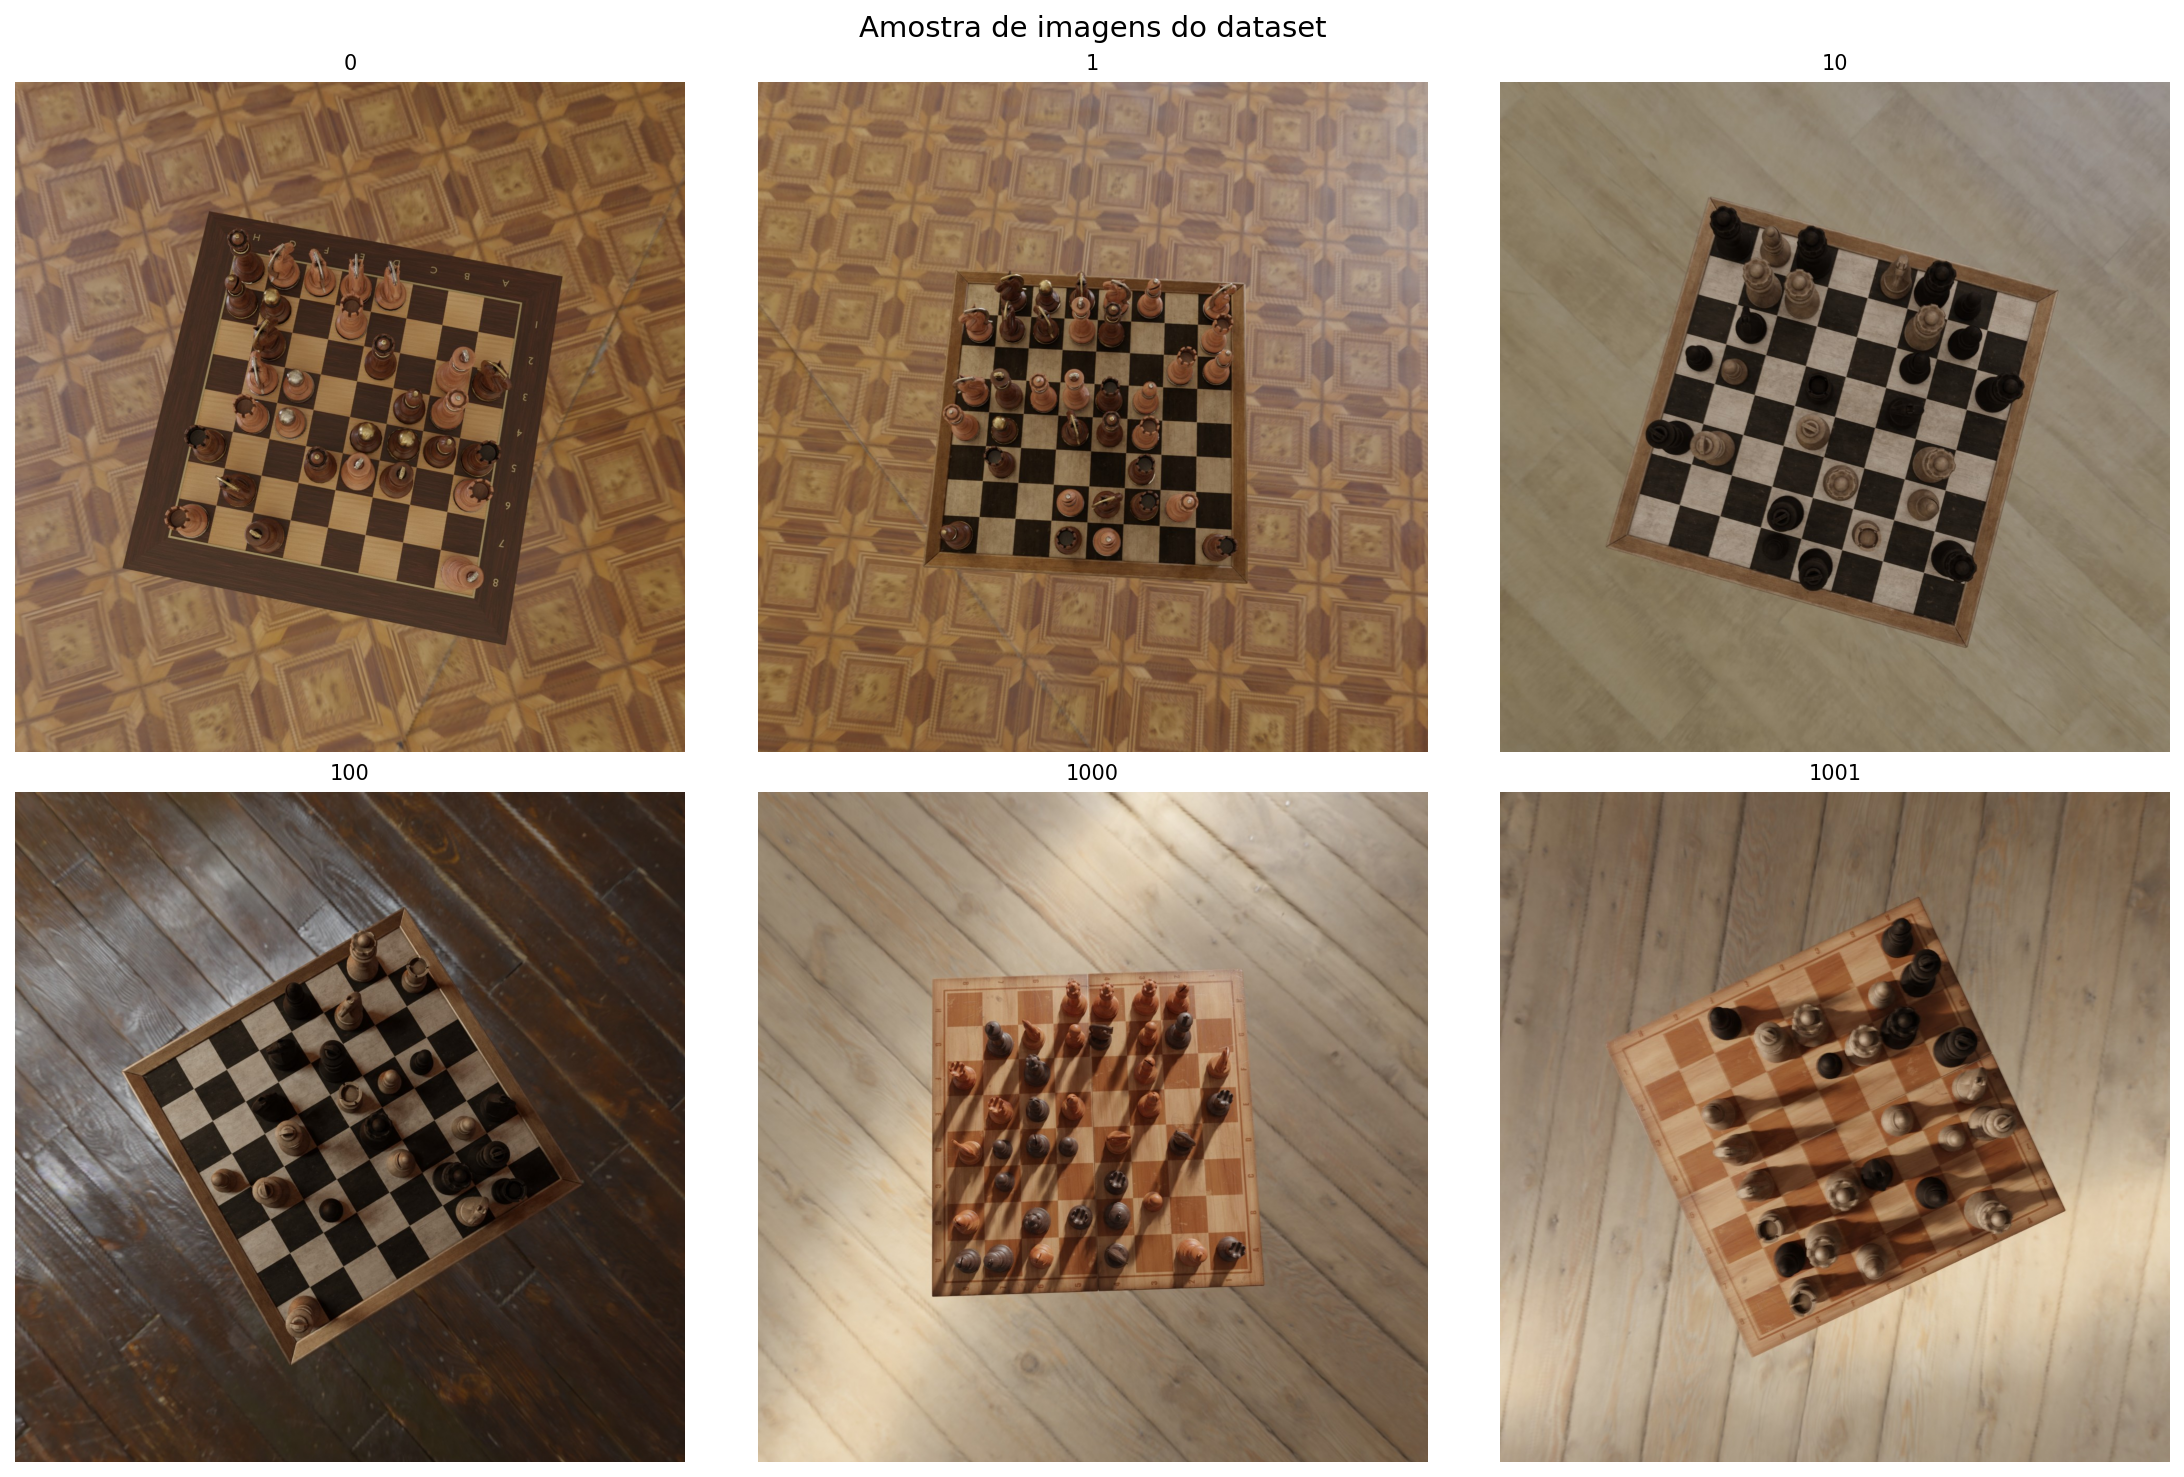
\includegraphics[width=0.85\linewidth]{../intro/images/01_dataset_samples.png}
\end{center}
}

\block{Pipeline Clássica}{
\begin{center}
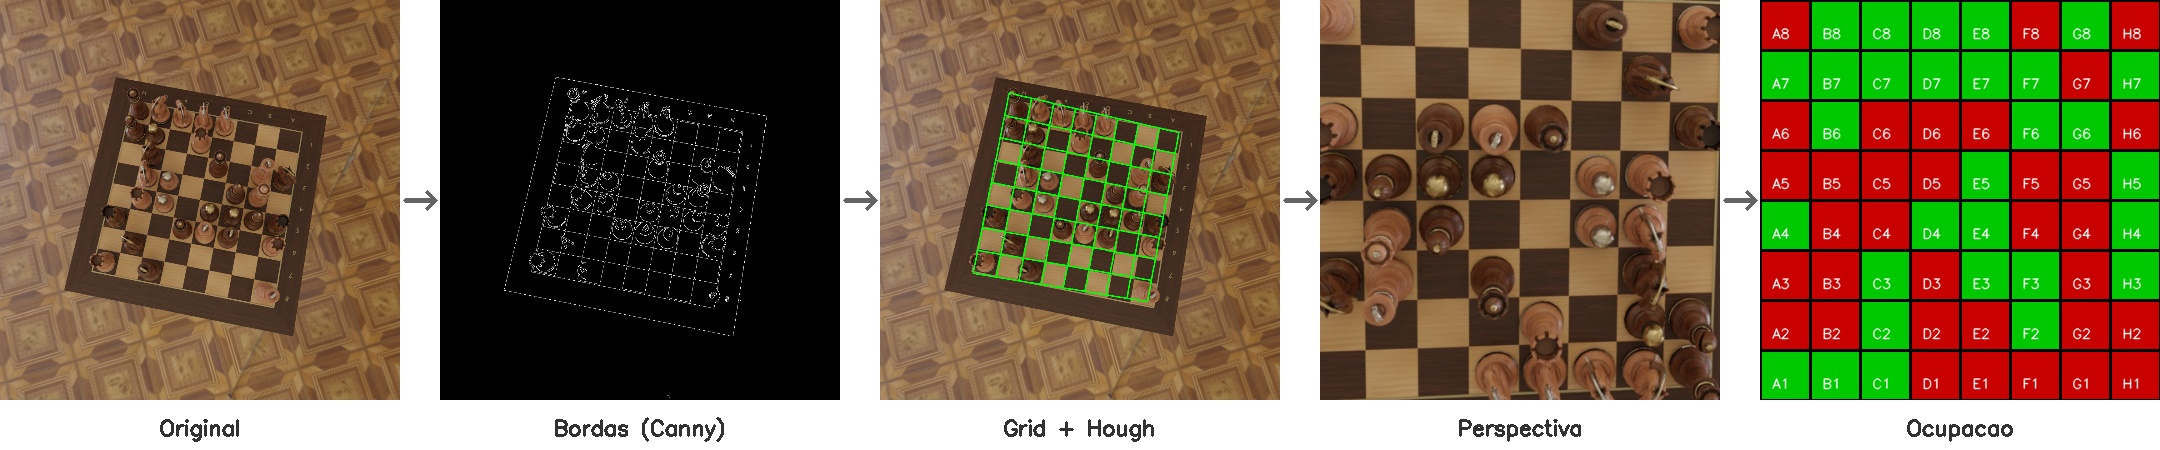
\includegraphics[width=0.95\linewidth]{../intro/images/slide_pipeline.jpg}
\end{center}
\vspace{0.3em}
Pré-processamento (cinza + blur gaussiano) $\rightarrow$ bordas (\textbf{Canny},
low=50/high=150) $\rightarrow$ linhas de grade (\textbf{Hough}) $\rightarrow$
\textbf{homografia} (vista de cima $480{\times}480$) $\rightarrow$ segmentação
$8{\times}8$ (casas de $60{\times}60$px).
}

\block{Ocupação e Cor (Clássico)}{
4 descritores por casa, combinados por votação ($\geq$2 de 4): desvio-padrão
de intensidade, densidade de bordas, variância do Laplaciano, diferença
centro-borda. Cor: limiar do canal V (HSV).

\begin{center}
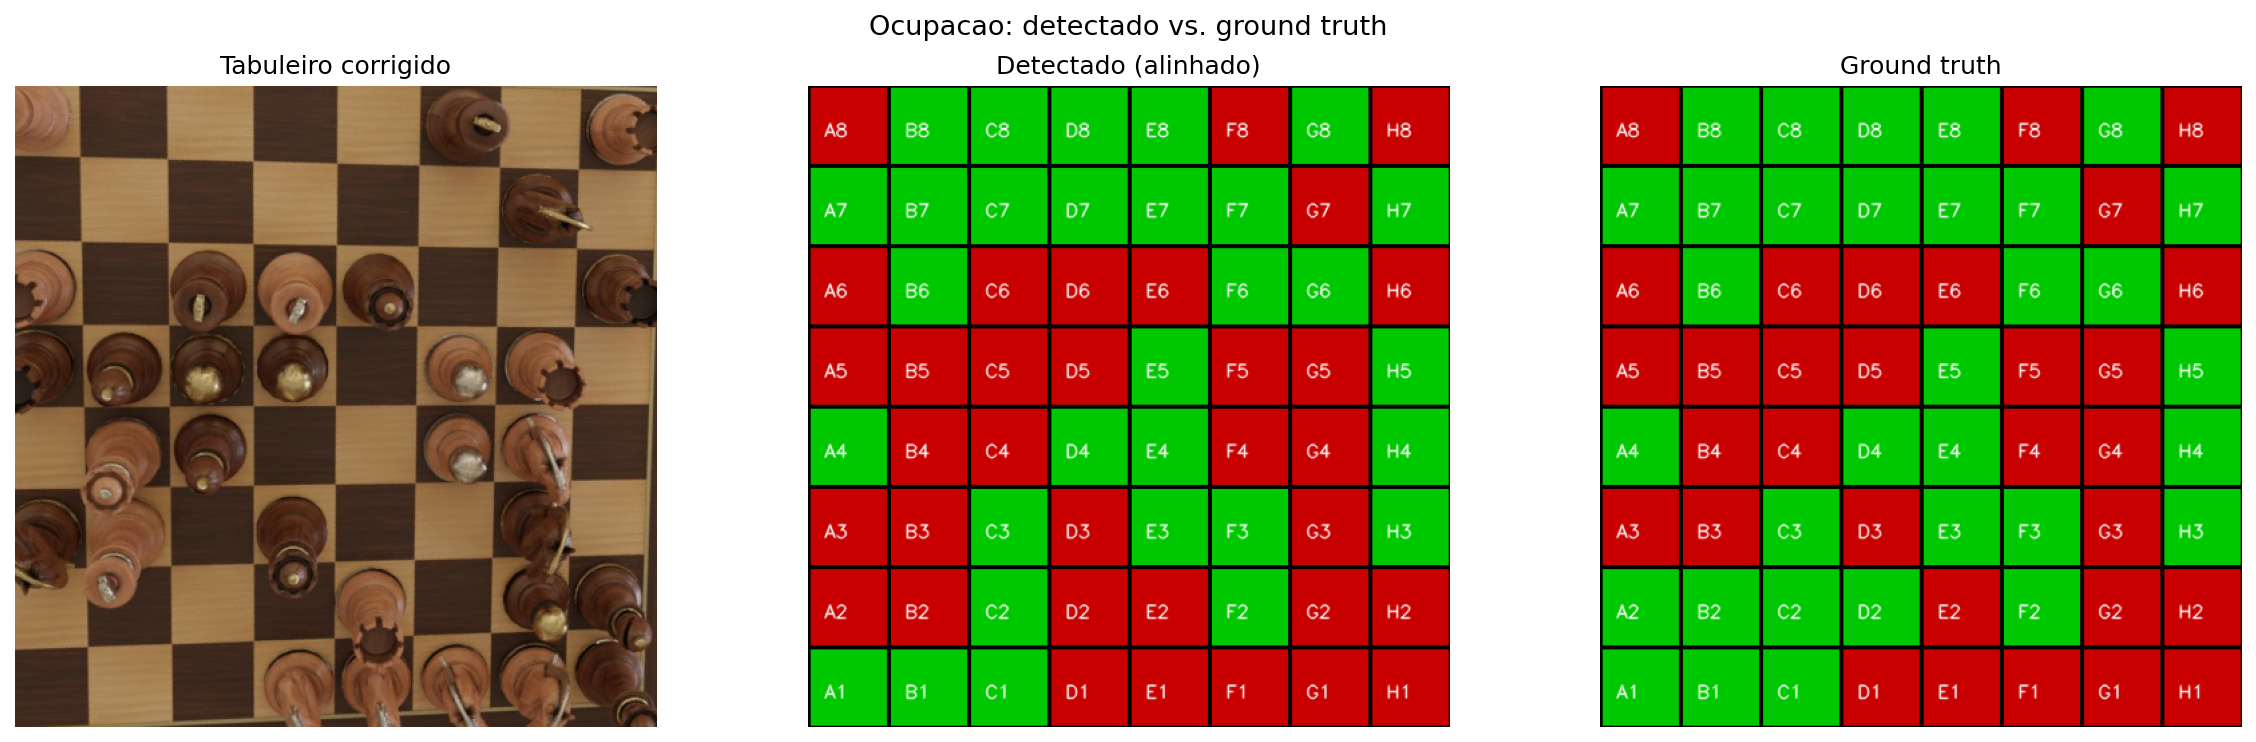
\includegraphics[width=0.85\linewidth]{../intro/images/10_occupancy_comparison.png}
\end{center}
}

% =========================================================== COLUMN 2 ======
\column{0.5}

\block{Classificação de Tipo (ResNet-34)}{
\textbf{Transfer learning} em 2 fases a partir de pesos ImageNet:
\begin{enumerate}
  \item \textit{Transfer learning} (10 épocas): \textit{backbone} congelado,
        treina só a cabeça (12 classes)
  \item \textit{Fine-tuning} (15 épocas): treina a rede inteira, ideal para
        aprender os detalhes finos que distinguem cada peça
\end{enumerate}
Treinado sobre \textasciitilde62\,000 células rotuladas automaticamente a
partir do gabarito, com \textit{augmentation} (flips, rotação $\leq$15\degree,
jitter de cor).

\begin{center}
\colorbox{mdSecondary}{\color{white}\bfseries\Large\strut~~F1 = 91\% em tipo de peça~~}
\end{center}

\begin{center}
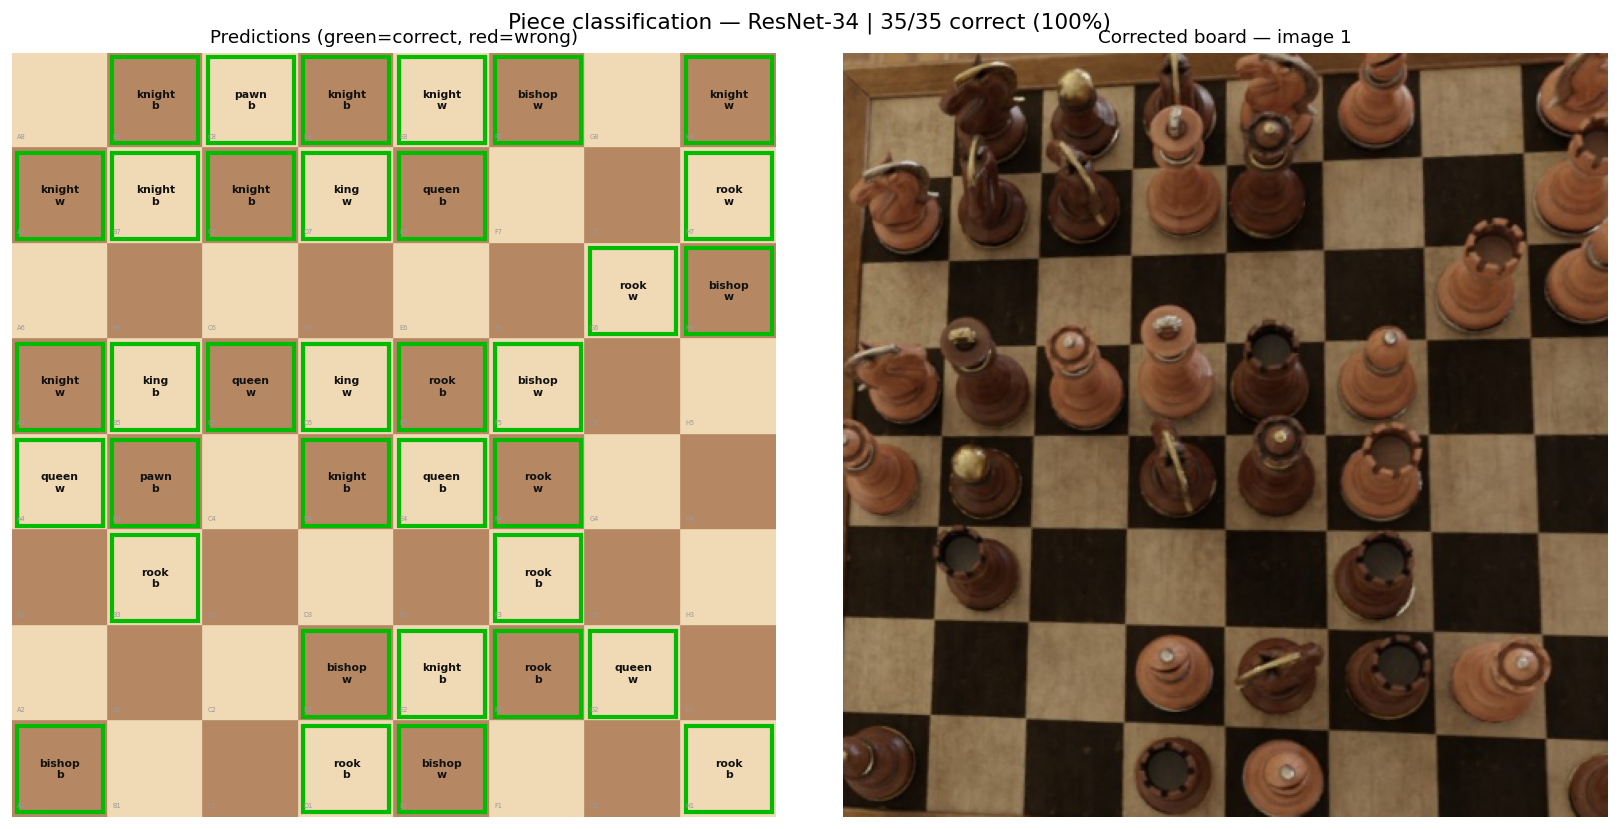
\includegraphics[width=0.7\linewidth]{../andamento/images/15_piece_classification_result.png}
\end{center}
}

\block{FEN e Detecção de Jogadas}{
A posição é serializada em FEN \textbf{completa} (6 campos). Leitura sem GT
fixa o \textbf{eixo} do tabuleiro (0\% erro), mas a simetria de cor sob
$180\degree$ deixa \textasciitilde42\% das leituras invertidas. Um algoritmo
determinístico infere lances em notação UCI a partir da comparação entre dois
estados: captura, roque, \textit{en passant}, promoção.
}

\block{Resultados}{
\begin{center}
\small
\begin{tabular}{@{}p{0.4\linewidth}p{0.5\linewidth}@{}}
\toprule
\textbf{Componente} & \textbf{Resultado} \\
\midrule
Ocupação (ponta a ponta) & F1 = 62,7\% (86,3\% c/ cantos GT) \\
Cor da peça (HSV) & 82,5\% \\
\textbf{Tipo da peça (ResNet-34)} & \textbf{F1 = 91,0\%} \\
Orientação (sem gabarito) & Lado do tabuleiro sempre correto; \textasciitilde42\% saem de cabeça para baixo \\
\bottomrule
\end{tabular}
\end{center}
\vspace{0.4em}
O gargalo de ponta a ponta é a detecção automática dos \textbf{4 cantos} do
tabuleiro sob baixo contraste; a votação de ocupação e o classificador de
tipo, que hoje é a etapa mais precisa do sistema, não são o problema.
}

\block{Referências}{
\footnotesize
He et al. (2016) \textit{Deep Residual Learning for Image Recognition}, CVPR.
\quad
Canny (1986) \textit{A Computational Approach to Edge Detection}, IEEE PAMI.
\quad
Duda \& Hart (1972) \textit{Use of the Hough Transformation...}, CACM.
}

\block{Conclusão}{
Visão clássica + Deep Learning (só onde o clássico falha) cobrem o problema de
ponta a ponta, da foto à jogada em notação.
}

\end{columns}

\end{document}
